\section{Introduction}
\label{sec:intro}

\textbf{Graphs are a natural model for relationships between entities}, and applications from social networks to fraud detection now routinely store and analyze graphs with billions of nodes and trillions of edges~\cite{ubiquityLargeGraphsVLDB2017,ching2015oneTrillion,besta2020demystifying,gupta2024graphscale,zhou2025redtao}.
In practice, nodes and edges carry \emph{labels} that assign them a type (e.g., ``User,'' ``follows'') and \emph{properties} modeled as key-value attributes (e.g., \texttt{name}, \texttt{age}); together these form a \emph{property graph}~\cite{Angles_Arenas_Barceló_Hogan_Reutter_Vrgoč_2018}.
The topology alone---nodes and edges without labels or properties---is called the \emph{structural graph}.
This distinction matters because graph workloads divide along it: transactional (OLTP) queries operate on the property graph, reading and mutating labels and attributes with low latency, while analytical (OLAP) tasks such as PageRank, connected components, and shortest-path computations operate on the structural graph and must touch large portions, if not all, of it~\cite{tang2022taming,qiu2018real}.

\textbf{Graph data management is split between two incompatible worlds.}
Graph databases such as Neo4j~\cite{neo4j} and ArangoDB~\cite{arangodb} store property graphs persistently and serve OLTP workloads well, but perform poorly on whole-graph analytics.
Purpose-built graph processing systems such as Ligra~\cite{shun2013ligra}, GraphChi~\cite{kyrola2012graphchi}, and Pregel~\cite{malewicz2010pregel} deliver orders-of-magnitude better OLAP performance, but require a costly extract-transform-load (ETL) pipeline to materialize the structural graph from the primary data store before any analysis can begin.
\textit{This is the central dichotomy of graph data management}: persistent storage with transactional guarantees, or fast analytics with an ETL tax---but not both.

\textbf{Existing attempts to bridge this gap fall short.}
One line of work keeps graphs in relational tables and routes analytics to a separate in-memory engine: Facebook's TAO~\cite{bronson2013tao} serves the social graph from MySQL but delegates analytics to offline pipelines; Oracle loads relational property graphs into PGX, an in-memory graph server, for analysis~\cite{OraclePG,WhatIsOracleSpatialGraph:online,hong2015pgx,welc2013graph,graphProcessingRDBMS,hong2013early}.
SQL/PGQ extensions~\cite{duckpgq:online} let users express pattern matching and path queries over relational tables, but build only transient in-memory representations and lack persistent graph layouts or transactional mutation support.
In both cases, traversals reduce to recursive self-joins whose cost grows with path length~\cite{10.1145/3129246,TransitiveClosureBiskupStiefeling1989}, and analytics still requires a dedicated in-memory engine or an ad-hoc construction step.

Hybrid Graph Transactional and Analytical Processing (HGTAP) systems are a more recent attempt to unify these workloads.
LiveGraph~\cite{zhu2019livegraph} stores adjacency lists in a large memory-mapped region, but its transaction manager serializes writers and limits both insertion throughput and OLAP scalability~\cite{libinzhou2025GTX,crotty2022you}.
GART~\cite{shen2023bridging} constructs an in-memory multi-versioned CSR bounded by main-memory capacity.
Neither system handles the full spectrum of operating conditions that real graph workloads demand.

\textbf{We make five observations about the graph data management landscape} that guide the design of our system:
\begin{enumerate}
  \item \textit{Layout construction dominates analytics cost.} The vast majority of time in graph analytics is spent creating the in-memory or on-disk data layout, not running the algorithm itself.
  \item \textit{Transaction management is expensive to build from scratch.} Supporting dynamic graphs requires ACID transactions, crash recovery, and concurrency control---substantial engineering that every new system must reimplement.
  \item \textit{No single operating regime suffices.} In-memory systems cannot handle graphs that exceed RAM; out-of-core systems sacrifice speed; distributed processing incurs severe communication overhead~\cite{mcsherry2015scalability,beamer2016understanding} and poor work balance~\cite{hajidehi2023cuttana}. A practical system must perform well across all three regimes.
  \item \textit{Data layout is the key determinant of performance.} An analytics-friendly persistent layout that preserves scan locality can serve both OLTP and OLAP workloads, and can be extended to store full property graphs with typed, columnar storage.
  \item \textit{Build on proven infrastructure, not from scratch.} A mature, production-quality key-value store already provides the transaction manager, write-ahead log, buffer pool, and out-of-core paging that a graph database needs. Building on such a foundation avoids years of storage-engine engineering and yields a system that is correct and performant from day one.
\end{enumerate}

\textbf{\project{} is a hybrid transactional and analytical graph database built on the \wt{}~\cite{WiredTigerDocumentation} key-value store.}
By encoding analytics-friendly graph layouts---adjacency lists and a CSR approximation---as sorted key ranges in \wt{}, \project{} inherits crash recovery, MVCC concurrency control, and buffer-pool management at no additional engineering cost, while delivering sequential scan performance that matches purpose-built in-memory systems.
\project{} extends its structural layouts with a typed property storage layer supporting both embedded and columnar storage modes.
On 20 LDBC SNB queries, \project{} achieves property-mutation latencies three to four orders of magnitude lower than Neo4j~\cite{neo4j} and JanusGraph~\cite{janusgraph}.
Insertion throughput scales near-linearly to 72 threads, sustaining up to 1.48\,M edges/sec on the write-optimized layout ($3\times$ higher than LiveGraph~\cite{zhu2019livegraph}).
\preliminary{Concurrent insertion and analytics results show that analytics latency remains competitive at moderate write ratios, with \project{} sustaining $1.8\times$ the mixed-workload write throughput of LiveGraph at the balanced operating point.}
We modified the GAP Benchmark Suite (GAPBS)~\cite{beamer2015gap} to use our iterator API and show that \project{}'s end-to-end analytics performance matches in-memory systems while scaling to out-of-core graphs.
\autoref{fig:fg-spider} summarizes these results: \project{} delivers robust performance across the entire spectrum of operating conditions---in-memory and out-of-core, static and dynamic, structural and property graph workloads---where every other system we evaluate covers only a subset.

\begin{figure}[t]
  \centering
  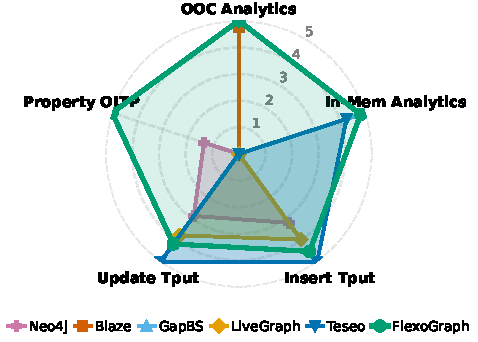
\includegraphics[scale=0.60]{content/fig/spider_chart.pdf}
  \caption{\project{} delivers robust performance across the entire spectrum of operating conditions common in graph data management. Each axis represents a workload class; points closer to the boundary indicate better performance relative to the best system in that class.}
  \label{fig:fg-spider}
\end{figure}

\textbf{Our contributions} are as follows.
\begin{itemize}
  \item The design of \project{}, a hybrid graph database built on \wt{} that unifies OLTP and OLAP graph workloads in a single persistent store without ETL or preprocessing (\autoref{sec:architecture}).
  \item An analysis of how adjacency-list and CSR-like layouts can be encoded as sorted key ranges in a key-value store to preserve scan locality for analytics (\autoref{arch:structural-reps}).
  \item A typed property storage layer with embedded and columnar modes that achieves property-mutation latencies three to four orders of magnitude lower than Neo4j, JanusGraph, and ArangoDB (\autoref{sec:evaluation}).
  \item Read-only snapshot iterators for analytics algorithms, with a flexible partitioning strategy that splits work between threads by vertex count or edge count (\autoref{arch:structural-reps}).
  \item An evaluation showing that \project{} matches the analytics performance of in-memory and out-of-core graph processing systems, scales insertion throughput near-linearly to 72 threads ($3\times$ LiveGraph), and delivers the transactional performance of in-memory dynamic graph containers (\autoref{sec:evaluation}).
\end{itemize}
